\chapter{Постановка требований и функциональности проекта}\label{ch:ch2}
% \section{Описание бизнес-ролей}\label{sec:ch2/sec1}


\section{Функциональные требования}\label{sec:ch2/sec2}
% \subsection{Основные требования}\label{sec:usecase_umls}

\subsection{Панель оператора}\label{sec:operator_control}
Панель оператора должна позволять пользователю с определёнными правами оператора производить действия связанные с управлением заказов, формированием отчётов и управлением списка конфигураций. Так же оператор должен иметь возможность работать со списком пользователей их аккаунтов и заказов и иметь возможность следить за выставляемыми клиентам счетами.

Для реализации необходимы страницы:
\begin{itemize}
  \item со списком клиентов;
  \item расширенной страницы клиента для оператора;
  \item оформления отчётов;
  \item редактирования списка конфигураций;
  \item списка выставленных счетов.
\end{itemize}

\subsection{Управление пользователями}\label{sec:users_control}
Для разделения прав пользователей должна быть реализована система разделения возможностей пользователей на основаниих их ролей.

Пользователь должен принадлежать одной определённой роли, что должно позволить системы быть проще, чем если бы была необходима более сложная система разделения прав на основании ролей. 

На таблице ~\ref{tab:roles} указаны основные типа ролей.
\begin{table} [htbp]% Пример записи таблицы с номером, но без отображаемого наименования
  \centering
  \begin{threeparttable}% выравнивание подписи по границам таблицы
    \caption{Список ролей пользователей}%
    \label{tab:roles}%
    \setlength\extrarowheight{4pt} %вот этим управляем расстоянием между рядами, \arraystretch даёт неудачный результат
    \setlength{\tymin}{1.9cm}% минимальная ширина столбца
    \begin{SingleSpace}
      \begin{tabulary}{\textwidth}{|@{}| >{\zz}C | >{\zz}C @{} |}
        \hline
        Роль & Описание \\ \hline
        Клиент & Пользователь имеет возможность оформлять заказы и работать с ним в рамках ограниченных операций.  \\ \hline
        Оператор & Ползователь имеет возможность управлять заказами клиентов в случае возникновения вопросов или у проблем у клиентов, запрашивать отчёты и выставлять счета. \\ \hline
      \end{tabulary}%
    \end{SingleSpace}
  \end{threeparttable}
\end{table}

\subsection{Управление заказами ВМ}\label{sec:order_control}
У клиентов должна быть возможность создавать и выполнять минимальный список операции по управлению ВМ заказа поддерживаемый системой виртуализации.
Для ВМ должно быть реализовано хранение списка состояний. 

Клиент должен иметь возможность:
\begin{itemize}
  \item запустить ВМ;
  \item выключить ВМ;
  \item перезагрузить ВМ;
  \item пересоздать ВМ.
\end{itemize}

Для реализации необходимы страницы:
\begin{itemize}
  \item выбора конфигурацией заказа (вм);
  \item подтверждения выбора и непосредственного оформления заказа; 
  \item списка заказов пользователя;
  \item страница управления заказом.
\end{itemize}

На странице заказа ВМ должна быть описана конфигурация вм и её состояние.


Для упрощения системы и её эксплуатация не должно быть возможности сменить конфигурацию ВМ. 

\subsection{Тарификация заказов}\label{sec:order_tarif}

Тарификация заказов должна проводиться по тарифам конфигураций ВМ. Конфигурация может иметь несколько тарифов с разными ценами для разных тарифицируемых периодов. 


Периоды тарификации
\begin{itemize}
  \item 1 месяц;
  \item 3 месяца; 
  \item 6 месяцев;
  \item 12 месяцев.
\end{itemize}

\subsection{Требованяи к оплате}\label{sec:order_pay}
Система должна хранить только данных о тарифах и платах (чеках) клиентов, вся оплата должна происходить через интеграцию со сторонней системой.


В своём профиле клиент должен иметь возможность увидеть список своих платежей и их статус.


При создании платежа необходимо создавать снапшот заказа и его тарифа.

\subsection{Формирование отчётов}\label{sec:report_gen}
Должна быть реализована возможность формирования определённого ряда отчётов с определёнными фильтрами.

На таблице ~\ref{tab:filters} указаны обязательные фильтры.
\begin{table} [htbp]% Пример записи таблицы с номером, но без отображаемого наименования
  \centering
  \begin{threeparttable}% выравнивание подписи по границам таблицы
    \caption{Список фильтров для формирования отчёта}%
    \label{tab:filters}%
    \setlength\extrarowheight{4pt} %вот этим управляем расстоянием между рядами, \arraystretch даёт неудачный результат
    \setlength{\tymin}{1.9cm}% минимальная ширина столбца
    \begin{SingleSpace}
      \begin{tabulary}{\textwidth}{|@{}| >{\zz}C | >{\zz}C @{} |}
        \hline
        Фильтр & Описание \\ \hline
        Тип отчёта &  Выбор типа из списка\\ \hline
        Диапазон дат & Выбор диапазона дат в форме календаря \\ \hline
      \end{tabulary}%
    \end{SingleSpace}
  \end{threeparttable}
\end{table}

В системе должна быть возможность указывать типы полей значений и алгоритмы вычисления для них для обеспечения упрощения создания новых типов отчётов и специальных полей в них.


Отчёт должен формироваться в формате CSV и отправляться на электронную почту запрасившего его оператора. Стобцы отчёта должны быть определены на этапе разработки.

\section{Нефункциональные требования}\label{sec:ch2/sec3}
Система должна обладать следующими качествами:
\begin{itemize}
  \item используется язык Ruby
  \item используется фреймворк Ruby on Rails
  \item используется СУБД PostgreSQL
  \item используется Sidekiq для фоновых задач
  \item система разрабатывается для ОС семейства *nix
  \item используется сервер unicorn
  \item используется nginx в роли реверс-прокси
  \item используется система виртуализации OpenStack
  \item оплата производится через систему Яндекс.Касса
\end{itemize}

\section{Диаграммы прецедентов}\label{sec:ch2/sec4}
На рисунке~\ref{fig:umls_register_ucesace} показан сценарий регистрации нового клиента.
\begin{figure}[ht]
  \centerfloat{
    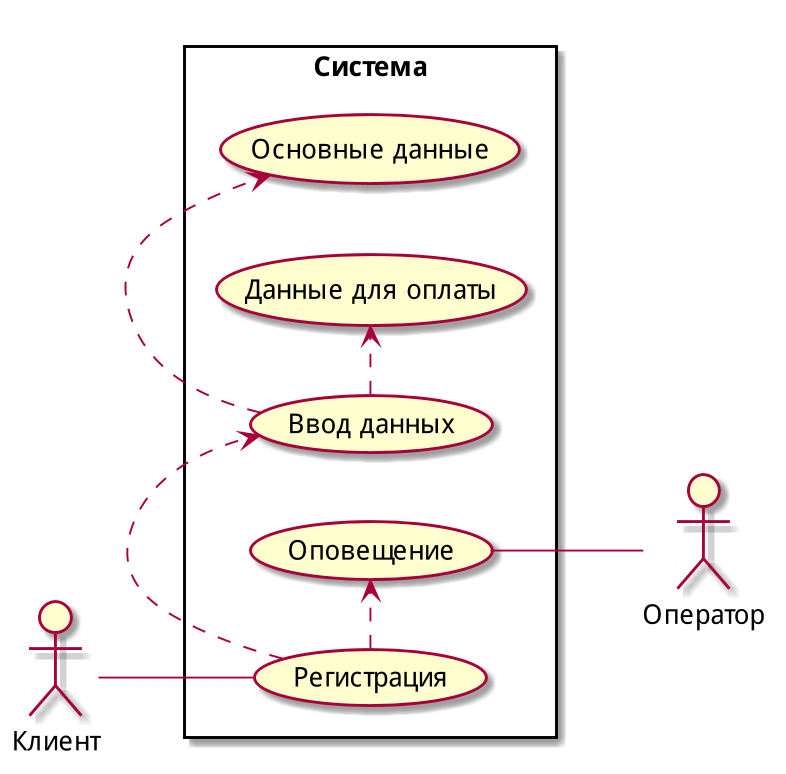
\includegraphics[scale=0.27]{umls/register_ucesace}
  }
  \caption{Сценарий регистрации клиента.}\label{fig:umls_register_ucesace}
\end{figure}

На рисунке~\ref{fig:umls_make_order_usecase} показан сценарий оформления заказа клиентом.
\begin{figure}[ht]
  \centerfloat{
    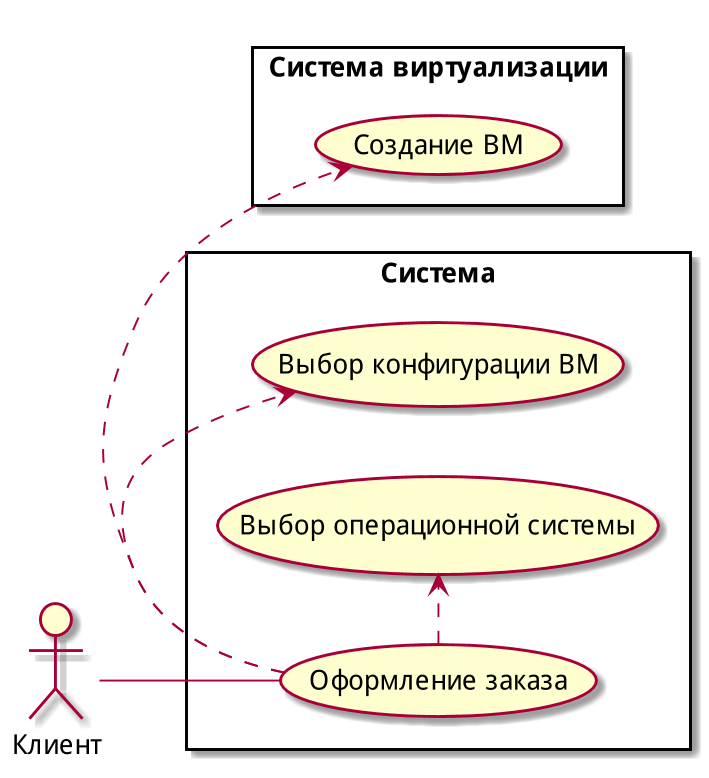
\includegraphics[scale=0.27]{umls/make_order_usecase}
  }
  \caption{Сценарий создания заказа.}\label{fig:umls_make_order_usecase}
\end{figure}

На рисунке~\ref{fig:umls_report_request_usecase} показан сценарий оформления заказа клиентом.
\begin{figure}[ht]
  \centerfloat{
    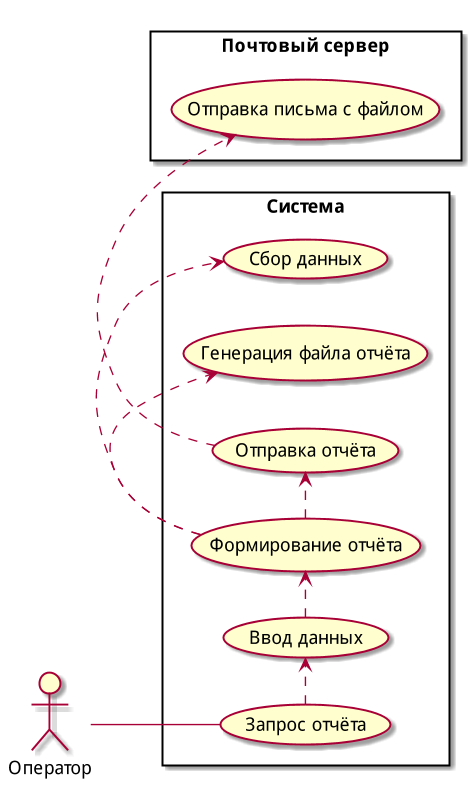
\includegraphics[scale=0.27]{umls/report_request_usecase}
  }
  \caption{Сценарий создания отчёта.}\label{fig:umls_report_request_usecase}
\end{figure}